\documentclass[11pt,a4paper]{article}
\usepackage{amsmath, graphicx, geometry, float}
\usepackage{hyperref, caption, subcaption}


\usepackage{typearea}
\areaset{160mm}{250mm}


\begin{document}
\title{\Large\bf Arbeit zum \\ \textit{Praktikum Mess- und Regelungstechnik} \\ Sommersemester 2022}
\author{Simon Klüpfel, Lukas Zeller \\
  Robotik und Telematik \\
  Universität Würzburg\\
  Am Hubland, D-97074 Würzburg\\
\small \texttt{lukas.zeller@stud.uni-wuerzburg.de} \\
\small \texttt{simon.kluepfel@stud.uni-wuerzburg.de}}
\date{Würzburg, 24.08.2022}

\maketitle

\section{Einleitungzum Volksbot-Roboter}
In dieser Arbeit befassen wir uns mit dem Robot Operating System, kurz \textit{ROS}, und der 
Verwendung dessen auf einem einfachen Roboter, dem \textit{Volksbot}. \\
Der verwendete Roboter ist der \textit{RT3-2} mit zwei passiven Rädern und der \textit{RT-3} mit einem passiven Rad.
Entwickelt wurden diese vom \textit{Fraunhofer Institut IAIS} aus Sankt Augustin. \\
Die technischen Daten sind wie folgt: \\
\vspace{-5mm}
\begin{center}
\begin{tabular}{| p{5cm} p{5cm} |}
  \hline
  Abmessungen & 580x520x315mm (L x B x H) \\
  Gewicht & 17kg \\
  
  Raddurchmesser & 260x85mm (aktive Räder) \\
   & 200mm (passive Räder) \\
  Maximale Geschwindigkeit & 2,2 $\frac{m}{s}$ \\
  
  Maximale Zuladung & 25kg \\
  \hline
\end{tabular} \\
\small{ Auszug aus \url{https://www.volksbot.de/rt3-de.php}}
\end{center}
Auf dem Roboter ist ein Laserscanner sowie Hardware zur Verbindung mit dem verwendeten
Laptop installiert. Außerdem lässt sich der Roboter über einen Joystick, ähnlich eines Gamecontrollers, manuell steuern. 
Wir verwenden sowohl vorgegebene ROS-Nodes, die uns von Institut für Robotik und Telematik zur Verfügung gestellt wurden, als auch angepasste Nodes die wir selbst erstellt beziehungsweise
geändert haben. 

\newpage

\section{Kartierung mit GMapping}
Wir starten zuerst die Node zur Kommunikation mit dem Roboter: \begin{verbatim}
  roslaunch volksbot messtechnikpraktikum.launch
\end{verbatim}
Um den Roboter zu steuern mit dem Controller benötigen wir die zugehörige Node: \begin{verbatim}
  roslaunch volksbot localjoystick.launch
\end{verbatim}
Nun erstellen wir eine \textit{rosbag}, die alle Topics des Roboters aufzeichnet: \begin{verbatim}
  rosbag record -a
\end{verbatim}
Um nun eine Karte erstellen zu können, müssen wir die aufgenommene \textit{bag} abspielen. 
Wichtig hier ist es den Parameter \begin{verbatim}
  rosparam set use_sim_time true
\end{verbatim} zu setzen um die Zeit aus dem \textit{clock}-Topic zu nutzen anstelle der globalen Systemzeit.
Nun kann man aus den Laserscanner-Daten, also hauptsächlich dem \textit{LMS}-Topic, die Map
erstellen. Hierzu starten wir das GMapping-Tool via \begin{verbatim}
  roslaunch volksbot messtechnikgmapping.launch
\end{verbatim}
Die Bag kann dann abgespielt werden mit \begin{verbatim}
  rosbag play filename.bag --clock
\end{verbatim}
Der \textit{clock}-Befehl am Ende ist wichtig um die Aufnahmen der \textit{rosbag} mit einem 
Zeitstempel zu versehen damit der Roboter sie nicht verwirft. 
Startet man nun RViz kann man über das \textit{map}-Topic den Aufbau der Map betrachten.
Um diese zu speichern startet man eine \textit{ROS-node} die das \textit{map}-Topic in
eine Datei speichert. 

\begin{figure}[H]
  \caption*{Abbildung 1: Aufgezeichnete Karte des Informatik-Untergeschosses}
  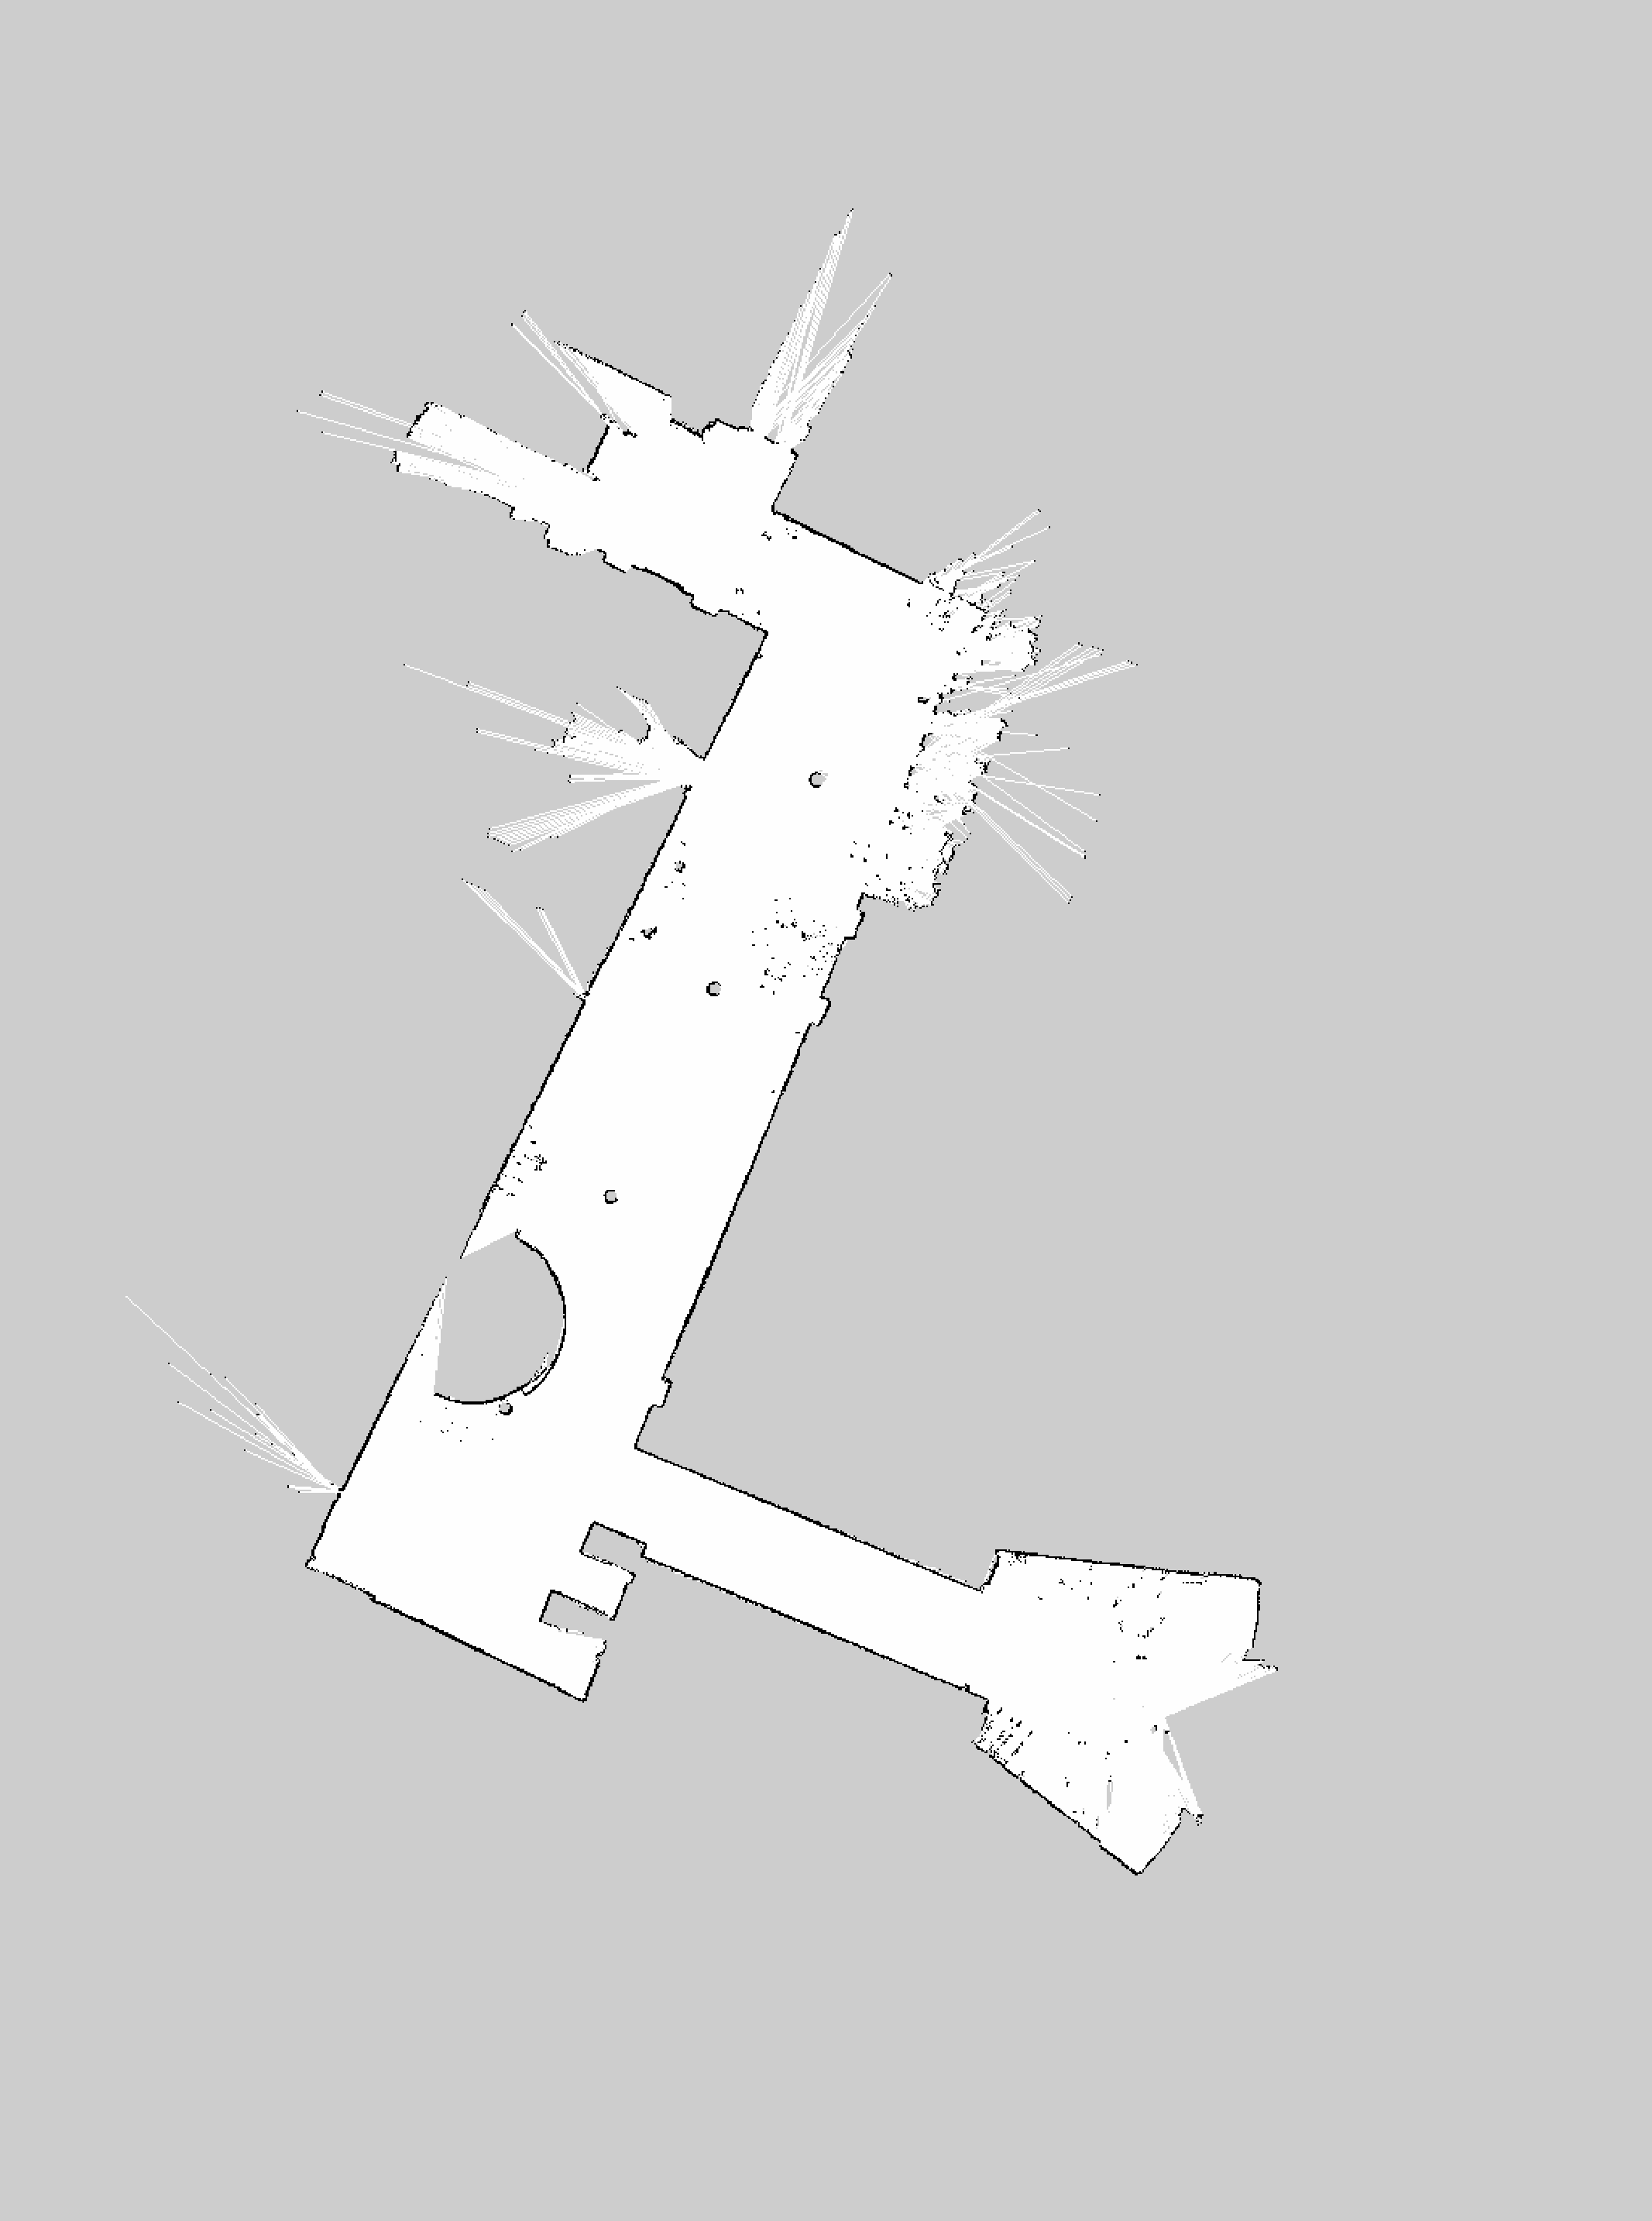
\includegraphics[scale = 0.3, angle = 90]{map.pdf}
  \centering
\end{figure}

% KOM: das ist falsch. zuerst fahren wir daten in eine Bag und machen aus der bag ne map


% KOM: wir brauchen dazu keine plots??? Wir haben nicht mal relevante. Ein bild der karte die wir rausbekommen haben reicht

\section{AMCL-Lokalisierung}
todo: vergleich AMCL-Odometrie

\section{Pfadverfolgung}
Pfade vergleichen, was gut, was schlecht, eventuell Code-Kommentare 

% KOM: du musst auf die Koordinatensysteme von AMCL/Odom eingehen. Das ist das Hauptthema im Code.

\section{Auswertung}
todo: 
Testen Sie den Regler mit dem aufgenommenen Pfad aus dem Informatikgebäude. Vergleichen Sie das Verhalten, wenn einmal die Odometrie und einmal die von AMCL bestimmten
Positionen als Messwerte für die Regelung verwendet werden.

also: plots, kommentare, was ist besser, was schlechter?

% KOM: An Plots brauchen wir hier Simulation, den rohen Pfad, AMCL, Odom, und Bilder was er IRL jeweils getan hat. Die Bilder kann ich noch machen.
\end{document}

